\section{Research Predictions}
\label{sec:research_predictions}

\subsection{Semi-supervised Learning}

{\bf Prediction:} Semi-supervised learning is here to stay. In particular,
self-supervised pretrained models will be a part of many machine-learning
applications, including speech recognition.

Part of my job as a research scientist is hiring, which means a lot of
interviews. I've interviewed more than a hundred candidates working on a
diverse array of machine-learning applications. Some large fraction,
particularly of the natural language applications, rely on a pretrained model
as the basis for their machine-learning enabled product or feature.
Self-supervised pretraining is already pervasive in language applications in
industry. I predict that by 2030 self-supervised pretraining will be just as
pervasive in speech recognition.

The past three years of deep learning have been the years of semi and
self-supervision. The field has undoubtedly learned how to improve
machin-learning models using unannotated data. Self-supervised
learning~\cite{lecun2021self} has benefited many of the most challenging
machine learning benchmarks. In language tasks, state-of-the-art records have
been repeatedly set and surpassed by self-supervised
models~\citep{devlin2019bert, radford2019language, yang2019xlnet}. Self and
semi-supervision are now commonplace and setting records in computer
vision~\citep{he2020momentum, chen2020simple, grill2020bootstrap}, abstractive
summarization~\citep{zhang2020pegasus} and machine
translation~\citep{sennrich2016improving}.

Speech recognition has also benefited from semi-supervised learning. Two
approaches are commonly used, both of which work well. The first approach is
self-supervised pretraining~\citep{schneider2019wav2vec, zhang2020pushing} with
a loss function based on contrastive predictive
coding~\citep{oord2018representation}. The idea is simple: train the model to
predict the future frame(s) of audio given the past. Of course, the devil is in
the details and the scale. The second approach is
pseudo-labeling~\citep{lee2013pseudo, kahn2020self, xu2020iterative}. Again the
idea is simple: use the trained model to predict the label on unlabeled data,
then train a new model on the predicted labels as if they were the ground
truth. And again the devil is in the details and the scale. The fact
that pseudo-labeling leads to better models is remarkable. It feels as if we
are getting something for nothing, a free lunch. The reason and the regime in
which pseudo-labeling works are interesting research questions.

The main challenges with self-supervision are those of scale, and hence
accessibility. Right now only the most highly endowed industry research labs
(\emph{e.g.} Google Brain, Google DeepMind, Facebook AI Research, OpenAI,
\emph{etc.}) have the funds to burn on the compute required to research
self-supervision at scale. As a research direction, self-supervision is only
becoming less accessible to academia and smaller industry labs.

{\bf Research implications:} Self-supervised learning would be more accessible
given lighter-weight models which could be trained efficiently on less data.
Research directions which could lead to this include sparsity for
lighter-weight models, optimization for faster training, and effective ways of
incorporating prior knowledge for sample efficiency.

\begin{figure*}[ht!]
    \centering
    \begin{subfigure}[b]{0.48\textwidth}
    \centering
    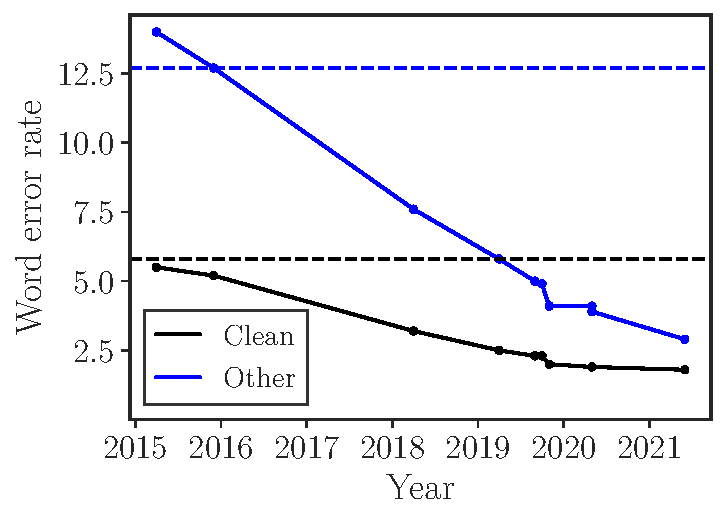
\includegraphics[width=\linewidth]{figures/librispeech_wer}
    \caption{LibriSpeech}
    \end{subfigure}
    \hfill
    \begin{subfigure}[b]{0.48\textwidth}
    \centering
    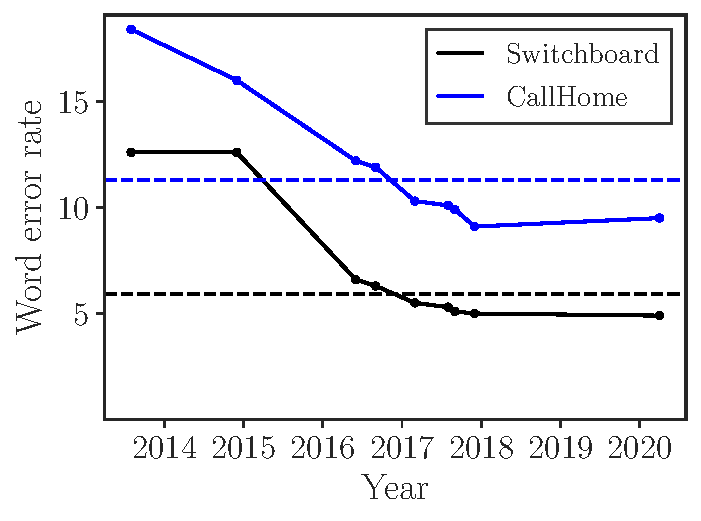
\includegraphics[width=\linewidth]{figures/switchboard_wer}
    \caption{Switchboard Hub5'00}
    \end{subfigure}
    \caption{The improvement in word error rate over time on the
    LibriSpeech~\citep{panayotov2015librispeech} and Switchboard Hub5'00
    benchmarks. The data for these figures is from
    \url{https://github.com/syhw/wer_are_we}. The dashed lines indicate
    human-level performance. The human-level results on LibriSpeech are
    reported in \citet{amodei2016deep}, and those on Switchboard are reported in
    \citet{xiong2016achieving}.}
    \label{fig:wers}
\end{figure*}

\subsection{On Device}
\label{sec:on_device}

{\bf Prediction:} Most speech recognition will happen on the device or at the
edge.

There are a few reasons I predict this will happen. First, keeping your data on
your device rather than sending it to a central server is more private. The
trend towards data privacy will encourage on-device inference whenever
possible. If the model needs to learn from a user's data, then the training
should happen on the device.

The second reason to prefer on-device inference is latency. In absolute terms,
the difference between 10 milliseconds and 100 milliseconds is not much.  But
the former is well below the perceptual latency of a human, and the latter well
above~\citep{lago2004quest, levitin2000perception}.  Google has already
demonstrated an on-device speech recognition system with accuracy nearly as
good as a server-side system~\citep{he2019streaming}. The latency differences
are easily noticeable.\footnote{For an example of the perceptual difference in
latencies see the blog post on Google's on-device speech recognizer:
\url{https://ai.googleblog.com/2019/03/an-all-neural-on-device-speech.html}}
From a pragmatic standpoint, the latency of the server-side recognizer is
probably sufficient. However, the imperceptible latency of the on-device system
makes the interaction with the device feel much more responsive and hence more
engaging.

A final reason to prefer on-device inference is 100\% availability. Having the
recognizer work even without an internet connection or in spotty service means
it will work all the time. From a user interaction standpoint there is a big
difference between a product which works most of the time and a product which
works every time.

{\bf Research implications:} On-device recognition requires models with smaller
compute and memory requirements and which use less energy in order to preserve
battery life. Model quantization and knowledge distillation (training a smaller
model to mimic the predictions of a more accurate larger model) are two
commonly used techniques. Sparsity, which is less commonly used, is another
approach to generate lighter-weight models. In sparse models, most of the
parameters (\emph{i.e.} connections between hidden states) are zero and can be
effectively ignored. Of these three techniques, I think sparsity is the
most promising research direction.

I believe we have extracted most of the value that quantization has to offer.
Even in the unlikely best possible scenario of further reducing quantization
from 8-bit to 1-bit, we only get a factor-of-eight gain. With distillation, we
still have a lot to learn. However, I believe uncovering the mechanism through
which distillation works will subsequently enable us to train small models
directly rather than taking the circuitous path of training a large model and
then a second small model to mimic the large model.

This leaves sparsity as the most promising research direction for
lighter-weight models. As findings like the ``lottery ticket hypothesis''
demonstrate~\citep{frankle2018lottery}, we have a lot to learn about the role
of sparsity in deep learning. In theory, the computational gains from sparsity
could be substantial. Realizing these gains will require developments in the
software, and possibly hardware, used to evaluate sparse models.

Weak supervision will be an important research direction for on-device training
for applications, which typically require labeled data. For example, a users
interaction with the output of a speech recognizer or the actions they take
immediately afterward could be useful signal from which the model can learn in
a weakly-supervised manner.

\subsection{Word Error Rate}
\label{sec:wer}

{\bf Prediction:} By the end of the decade, possibly much sooner, researchers
will no longer be publishing papers which amount to ``improved word error rate
on benchmark X with model architecture Y''.

As you can see in figure~\ref{fig:wers}, word error rates on the two most
commonly studied speech recognition benchmarks have saturated. Part of the
problem is that we need harder benchmarks for researchers to study.  Two
recently released benchmarks may spur further research in speech
recognition~\citep{chen2021gigaspeech, galvez2021people}. However, I predict
that these benchmarks will quickly saturate by scaling up models and
computation.

Another part of the problem is that we have reached a regime where word error
rate improvements on academic benchmarks no longer correlate with practical
value. Speech recognition word error rates on both benchmarks in
figure~\ref{fig:wers} surpassed human word error rates several years
ago.\footnote{Estimates of human-level word error rates on the CallHome portion
of Hub5'00 vary considerably. For example \citet{saon2017english} report a best
result 6.8 out of three transcribers whose results vary by nearly 2.0 absolute
word error rate.} However, in most settings humans understand speech better
than machines do. This implies that word error rate as a measure of the quality
our speech recognition systems does not correlate well with an ability to
understand human speech.

A final issue is research in state-of-the-art speech recognition is becoming
less accessible as models and data sets are getting larger, and as computing
costs are increasing. A few well-funded industry labs are rapidly becoming the
only places that can afford this type of research. As the advances become more
incremental and further from academia, this part of the field will continue to
shift from research labs to engineering organizations.

\subsection{Richer Representations}

\begin{figure}
\centering
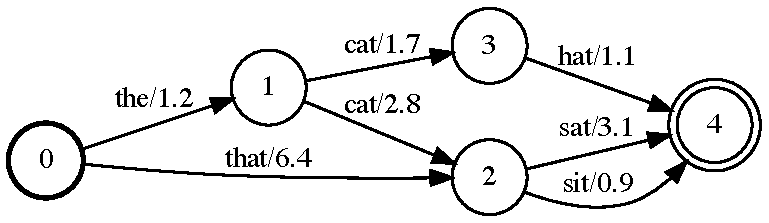
\includegraphics[width=\linewidth]{figures/lattice}
\caption{An example lattice used to encode mutliple hypotheses output from a
    speech recognizer with differing weights.}
\label{fig:lattice}
\end{figure}

{\bf Prediction:} Transcriptions will be replaced by richer representations for
downstream tasks which rely on the output of a speech recognizer. Examples of
such downstream applications include conversational agents, voice-based search
queries, and digital assistants.

Downstream applications often don't care about a verbatim transcription; they
care about semantic correctness. Hence, improving the word error rate of a
speech recognizer often does not improve the objective of the downstream task.
One possibility is to develop a \emph{semantic error rate} and use
it to measure the quality of the speech recognizer. This is a challenging
albeit interesting research problem.

I think a more likely outcome is to give downstream applications richer
representations from the speech recognizer. For example, instead of passing a
single transcription, passing a lattice of possibilities (as in
figure~\ref{fig:lattice}) which captures the uncertainty for each could be much
more useful.

{\bf Research implications:} The exact structure used to encode the
representation is an open question. One possibility could be some sort of
weighted transducer which if differentiable could allow for fine-tuning the
recognizer to specific applications~\cite{k2, hannun2020differentiable}. This
type of representation also requires models which are able to ingest
variable-sized graphs as input.

\subsection{Personalization}

{\bf Prediction:} By the end of the decade, speech recognition models will be
deeply personalized to individual users.

One of the main distinctions between the automatic recognition of speech and
the human interpretation of speech is in the use of context. Humans rely on a
lot of context when speaking to one another. This context includes the topic
of conversation, what was said in the past, the noise background, and visual
cues like lip movement and facial expressions. We have, or will soon
reach, the Bayes error rate for speech recognition on short (\emph{i.e.} less
than ten second long) utterances taken out of context. Our models are using the
signal available in the data to the best of their ability. To continue to
improve the machine understanding of human speech will require leveraging
context as a deeper part of the recognition process.

One way to do this is with personalization. Personalization is already used to
improve the recognition of utterances of the form ``call \texttt{<NAME>}''.
\citet{sim2019personalization} found personalizing a model with a user's
contact list improves named entity recall from 2.4\% to 73.5\% -- a massive
improvement. Personalizing models to individual users with speech disorders
improves word error rates by 64\% relative~\citep{sim2019investigation}.
Personalization can make a huge difference in the quality of the
recognition, particularly for groups or domains that are underrepresented in
the training data. I predict we will see much more pervasive personalization by
the end of the decade.

{\bf Research implications:} On-device personalization requires on-device
training which in itself requires lighter-weight models and some form of weak
supervision (see section~\ref{sec:on_device}).  Personalization requires models
which can be easily customized to a given user or context. The best way to
incorporate such context into a model is still a research question.
